\chapter{Experimentos}
\label{cha:experimentos}

Neste capítulo é avaliado o desempenho e o consumo energético de aplicações
\stencil do \pskel quando executadas no \mppa e em um processador Intel Xeon
E5-2640 v4 com 10 núcleos de 2.4GHz e 64GB de \ram (Broadwell). As medições de energia no \mppa
foram feitas considerando todos os \textit{clusters}, a memória, os subsistemas
de \es e a \noc, onde foram coletadas por meio dos sensores de potência e
energia disponíveis no \mppa. Como o \mppa possui características intrínsecas do
próprio processador que garante de baixa variabilidade entre as execuções, foram
realizadas somente 5 repetições de cada experimento, computando-se a média
aritmética dos valores. Todos os experimentos no \mppa consideraram 16
\pes por \textit{cluster}. Por outro lado, as medições de energia e tempo no
processador Intel com o uso do \rapl através da biblioteca PAPI~\cite{papi12}.
Em cada experimento foram utilizadas 10 \textit{threads} sem uso de
\textit{hyperthreading}. Os resultados mostram a média aritmética de 30
execuções. Por fim, todos os resultados mostraram um desvio padrão menor que
$1$\%.

Devido às limitações de memória em cada \textit{cluster}, ao ser especificado
uma quantidade muito grande de iterações, o \textit{tile} alargado pode ser
maior do que a memória presente em cada \textit{cluster}. Portanto, foi fixado
uma quantidade de 10 iterações internas para cada \textit{cluster}. Além disso,
para os experimentos terem uma quantidade significativa de sincronizações sobre
a execução de cada aplicação, foi adotado 30 iterações para cada aplicação.

\section{Aplicações \stencil}
\label{cha:aplicacoes}

Para a realização dos experimentos foram utilizadas as seguintes aplicações estêncil:

\textbf{Fur:} modela a formação de padrões sobre a pele de animais\footnote{{http://ccl.northwestern.edu/netlogo/models/Fur}}. Nessa aplicação, a pele do animal é modelada por uma \textit{array} bidimensional de células de pigmento que podem estar em um dos dois estados: colorida ou não-colorida. As células coloridas secretam ativadores e inibidores. Ativadores fazem uma célula central se tornar colorida; inibidores, por outro lado, fazem uma célula central se tornar não colorida.
A diferença entre as potências dos ativadores e inibidores é responsável por decidir a coloração da célula central, onde mais ativadores resulta em uma célula colorida e mais inibidores resulta em uma célula não colorida. Nos casos em que as potências dos ativadores e inibidores forem iguais, a cor da célula permanece inalterada. A máscara contém células adjacentes à célula central e seu tamanho é parametrizável. Neste trabalho foi utilizado $2$ vizinhos adjacentes em cada direção.

\textbf{Jacobi:} método iterativo para resolver equações matriciais~\cite{demmel97}.
O método converge garantidamente se a matriz de entrada é restrita ou irredutívelmente dominante diagonalmente, i.e., $|u_{i,i}| > \sum_{j\neq i}{|u_{i,j}|}$, para todo $i$.
A Equação~\ref{eq:JacobiPoisson} define a computação em cada passo do método iterativo de Jacobi para resolver a equação discreta elíptica de Poisson~\cite{demmel97}. A solução aproximada é computada discretizando o problema na matriz em pontos espaçados de forma equivalente por $n\times n$.\\
 \begin{equation}
 u'_{i,j} = \frac{u_{i\pm1,j} + u_{i,j\pm1} + h^2f_{i,j}}{4}
 \label{eq:JacobiPoisson}
 \end{equation}
 A cada passo, o novo valor de $u_{i,j}$ é obtida fazendo a média $h^2f_{i,j}$ dos seus vizinhos, onde $h = \frac{1}{n+1}$ e $f_{i,j} = f(ih,jh)$,
 para uma dada função $f$.

\textbf{GoL:} autômato celular que implementa o Jogo da Vida de Conway \cite{gardner70}. O autômato é representado por um \textit{array} bidimensional, onde cada elemento representa um indivíduo vivo ou um indivíduo morto. A máscara do estêncil, a qual determina a interação entre o indivíduo e seus vizinhos, considera as $8$ células vizinhas adjacentes à célula central. Dependendo dos valores dos vizinhos, o elemento pode modificar seu estado entre vivo e morto.\\

\begin{figure}[t]
	\centering
	\subfigure{\label{fig:furTileTime} 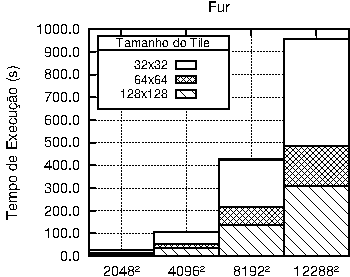
\includegraphics[width=0.4\textwidth]{figs/MPPAPlotfurTimeTiles.pdf}}
	\qquad
	\subfigure{\label{fig:golTileTime} 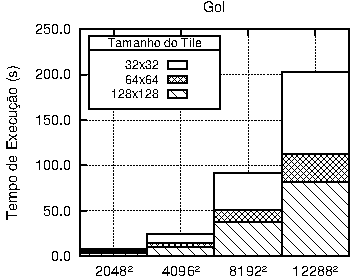
\includegraphics[width=0.4\textwidth]{figs/MPPAPlotgolTimeTiles.pdf}}
    \qquad
	\subfigure{\label{fig:jacobiTileTime} 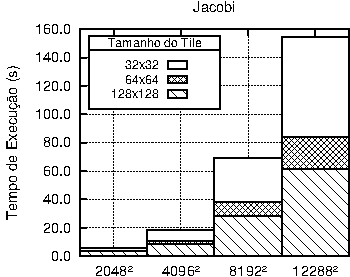
\includegraphics[width=0.4\textwidth]{figs/MPPAPlotjacobiTimeTiles.pdf}}
	\caption{Tempos de execução das aplicações para diferentes tamanhos de \textit{tile} e \texttt{Array2D} no \mppa.}
	\label{fig:timeBox}
\end{figure}

\begin{figure}[t]
	\centering
	\subfigure{\label{fig:furTileTime} 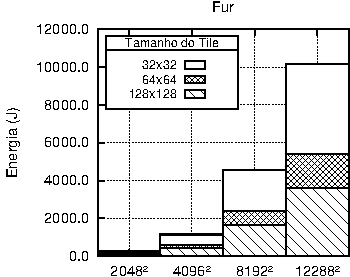
\includegraphics[width=0.4\textwidth]{figs/MPPAPlotfurEnergyTiles.pdf}}
	\qquad
	\subfigure{\label{fig:golTileTime} 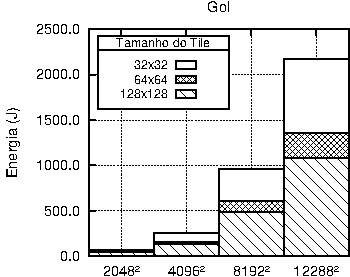
\includegraphics[width=0.4\textwidth]{figs/MPPAPlotgolEnergyTiles.pdf}}
    \qquad
	\subfigure{\label{fig:jacobiTileTime} 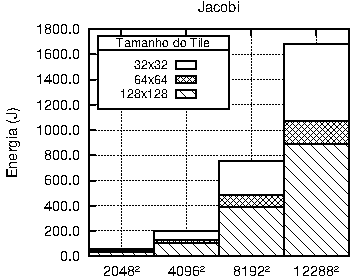
\includegraphics[width=0.4\textwidth]{figs/MPPAPlotjacobiEnergyTiles.pdf}}
	\caption{Consumo de energia das aplicações para diferentes tamanhos de \textit{tile} e \texttt{Array2D} no \mppa.}
	\label{fig:energyBox}
\end{figure}

\begin{figure}[t]
    \centering
    \subfigure[fig:comparisonTime][Tempo de execução.]{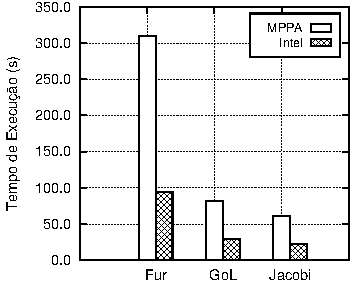
\includegraphics[width=0.4\columnwidth]{figs/ComparisonTimeTiles10.pdf}}
    \qquad
    \subfigure[fig:comparisonEnergy][Consumo de Energia.]{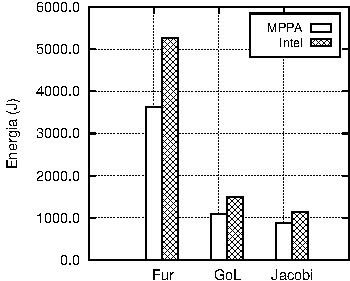
\includegraphics[width=0.4\textwidth]{figs/ComparisonEnergyTiles10.pdf}}
    \caption{Comparação do tempo de execução e consumo de energia das aplicações \textit{Fur}, \textit{GoL} e \textit{Jacobi} em relação a arquitetura.}
    \label{fig:comparison-time}
\end{figure}

\subsection{Impacto do Tamanho do \textit{Tile} no Desempenho do \mppa}

O primeiro experimento tem por objetivo verificar o impacto do tamanho dos
\textit{tiles} no desempenho e consumo energético das aplicações. As
Figuras~\ref{fig:timeBox} e \ref{fig:energyBox} mostram, respectivamente, os
tempos de execução e consumo de energia de três aplicações estêncil, variando-se
o tamanho do \texttt{Array2D} de entrada (de $2048^2$ até $12288^2$) e os
tamanhos do \textit{tile} (de $32^2$ até $128^2$). \textit{Arrays} de entrada
maiores que $12288^2$ e \textit{tiles} maiores que $128^2$ extrapolam às
memórias \lpddr e dos \textit{clusters}, respectivamente.

Pode-se perceber uma redução no tempo de execução à medida em que se aumenta o
tamanho do \textit{tile} (Figura~\ref{fig:timeBox}), pois há menos
sincronizações e comunicações de \textit{tiles} entre os processos mestre e
escravos. O comportamento das aplicações é similar, sendo diferenciado apenas
pela grandeza dos tempos de execução.
A Figura~\ref{fig:energyBox} apresenta um comportamento similar para o consumo
de energia, pois o tempo de execução reduz com o aumento do tamanho do
\textit{tile}, trazendo uma redução no consumo de energia.

\subsection{Análise de Escalabilidade no \mppa}

Em um segundo experimento, buscou-se verificar a escalabilidade das aplicações
no \mppa. Para isso, variou-se o número de \textit{clusters} em cada aplicação,
com \texttt{Array2D} de entrada fixo de tamanho $4096^2$ e \textit{tiles} de
tamanho $128^2$. A Figura~\ref{fig:appsTime} apresenta os tempos de execução
obtidos ao variar-se o número de \textit{clusters} utilizados na computação. A
Figura~\ref{fig:speedup}, por outro lado, apresenta o fator de aceleração
(\textit{speedup}) com relação ao tempo de execução com 1 \textit{cluster}. Em
outras palavras, o \textit{speedup} com $c$ \textit{clusters} é computado
dividindo-se o tempo de execução obtido com apenas 1 \textit{cluster} pelo tempo
de execução obtido com $c$ \textit{clusters}.

No geral, os resultados mostraram que a solução proposta para o \mppa é
escalável. Porém, pode-se notar que a aplicação \textit{Fur} apresentou uma
escalabilidade superior às demais aplicações. Esse comportamento está
diretamente relacionado com a quantidade de operações realizadas pelo
\textit{kernel} da aplicação (complexidade do \textit{kernel}). Tendo em vista a
necessidade de comunicações no \mppa, o tempo total de execução de uma aplicação
passa a ser composto pela soma do tempo de comunicação com o tempo de
computação. Para um dado \textit{tile} $t$ de tamanho fixo, o tempo necessário
para realizar comunicações de $t$ entre mestre e escravo será constante. Por
outro lado, quanto maior o número de operações (computações) feitas em $t$ pelo
\textit{kernel} da aplicação, maior será o paralelismo a ser explorado. Nesse
caso, o tempo de computação será proporcionalmente maior que o tempo de
comunicação, melhorando assim a escalabilidade obtida. Este é o caso da
aplicação \textit{Fur} cujo \textit{speedup} se aproxima do caso ideal. Em
contrapartida, aplicação \textit{Jacobi} apresentou uma escalabilidade mais
baixa que as demais, pois seu \textit{kernel} apresenta baixa complexidade.

\begin{figure}[t]
    \centering
    \subfigure[Tempo de execução.]{\label{fig:appsTime} 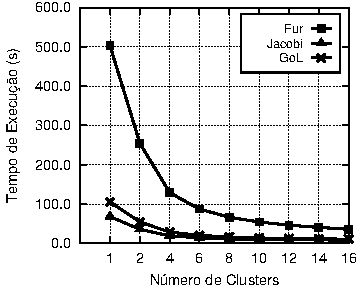
\includegraphics[width=0.4\textwidth]{figs/MPPAPlotScalability.pdf}}
    \qquad
    \subfigure[Speedup.]{\label{fig:speedup} 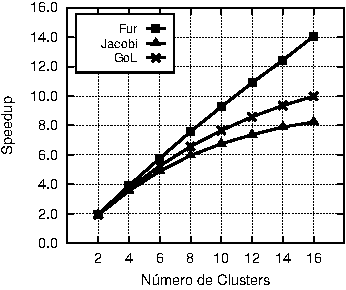
\includegraphics[width=0.4\textwidth]{figs/MPPAPlotSpeedup.pdf}}
    \caption{Resultados de tempo e \textit{speedup} das aplicações \textit{Fur}, \textit{GoL} e \textit{Jacobi}.}
    \label{fig:scalability}
\end{figure}

\subsection{Kalray \mppa vs. Intel Broadwell}

Por fim, foram efetuados experimentos comparativos entre o processador Intel
Xeon e o \mppa, como pode-se ver na Figura~\ref{fig:comparison-time}. Nesses
experimentos, utilizou-se um \texttt{Array2D} de entrada de tamanho $12288^2$ e
\textit{tiles} de tamanho $128^2$. Ao ser comparado o tempo das aplicações em
cada arquitetura, nota-se que o \mppa tem um desempenho pior, contudo ao ser
comparado o consumo de energia percebe-se um comportamento diferente: a energia
consumida pelo \mppa é menor, principalmente na aplicação \textit{Fur}. No
geral, o consumo de energia das aplicações \textit{Fur}, \textit{GoL} e
\textit{Jacobi} no \mppa foi aproximadamente $1.45$x, $1.38$x e $1.27$x menor
que no Intel Xeon, respectivamente. Por outro lado, o tempo de execução dessas
aplicações obtido no \mppa foi  $3.30$x, $2.83$x e $2.69$x maior que no Intel
Xeon, respectivamente.

%\begin{figure}[t]
%	\centering
%	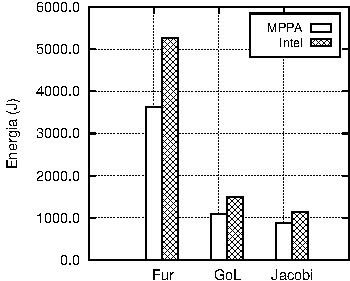
\includegraphics[width=0.4\columnwidth]{figs/ComparisonEnergyTiles10.pdf}\\
%	\caption{Comparação do consumo de energia das aplicações \textit{Fur}, Gol e Jacobi.}
%	\label{fig:comp-energy}
%\end{figure}

